\nchapter{Alphabet und Aussprache}


\section{System der Aussprache}
\noindent Das Na'vi verfügt über 20 Konsonanten, sieben Vokale und zwei silbische Sonoranten, die Frommer als ``Pseudovokale'' bezeichnet. \LanguageLog

\subsection{Konsonantismus}
Die Tabelle unten zeigt die Konsonanten des Na'vi. Phoneme in Klammern repräsentieren die Aussprache bestimmter Laute und Angleichungen, die im Riff-Na'vi vorkommen, jedoch keine eigene Schreibweise erhalten.

\begin{center}
	\begin{tabular}{llllll}
		& Labial & Alveolar & Palatal & Velar & Glottal \\
		Ejektive &	\N{px} [p'] & \N{tx} [t'] & & \N{kx} [k'] & \\
		Stimmlose Plosive & \N{p} [p] & \N{t} [t] & & \N{k} [k] & \N{’} [ʔ] \\
		Stimmhafte Plosive    &  ([b])    & ([d])    &  & ([g]) & \\
		Affrikaten &             & \N{ts}  [ts] & ([tʃ]) & & \\
		Stimmlose Frikative & \N{f} [f] & \N{s} [s] & ([ʃ]) & & \N{h} [h] \\
		Stimmhafte Frikative & \N{v} [v] & \N{z} [z] & & & \\
		Nasale &         \N{m} [m] & \N{n} [n] & & \N{ng} [ŋ] & \\
		Liquide &         &  \N{r} [ɾ], \N{l} [l] & & & \\
		Halbvokale (Gleitlaute) &       \N{w} [w] & &  \N{y} [j] & & \\
	\end{tabular}
\end{center}

\subsubsection{} Stimmlose Plosive am Anfang und in der Mitte eines Wortes sind nicht aspiriert. Sie sind zudem am Wortende ungelöst, sowie auch am Ende einer Silbe, wenn ein weiterer Konsonant folgt (z. B. in \N{txe\uwave{p}mì} und \N{'o\uwave{k}trr}). Folgt jedoch innerhalb eines Satzes ein Vokal auf einen Plosiv am Wortende, wird dieser bei natürlicher Aussprache gelöst, \N{oel se\uwave{t o}mum}. Ungelöste Plosive fallen am ehesten bei größeren Pausen auf, wie in \N{oel omum se\uwave{t}.}

\subsubsection{} Das \N{r} ist ein alveolarer Flap (Schlaglaut). Das \N{l} wird deutlich und im vorderen Bereich des Mundes (alveolar) artikuliert, so wie in ``Laub'', im Gegensatz zum ``dunklen'' l ([ɫ]) aus dem Englischen, z. B. in ``call''.

\subsubsection{}Frommer entwickelte eine wissenschaftliche Schreibweise, in der zwei der Digraphen als ein einziger Buchstabe geschrieben wurden, \N{c} für \N{ts} und \N{g} für \N{ng}. Das Digraphensystem war für die Schauspieler einfacher, es wurde aber auch von Frommer in Medieninterviews und in den meisten seiner eigenen E-Mails benutzt. Die wissenschaftliche Schreibweise findet sich nur in einigen frühen E-Mails an und von Frommer.  \label{lands:cg}

\subsubsection{} Da einfache Plosive als Silbenende verwendet werden können, ist die gebräuchlichere Schreibweise für Ejektive, \N{p'}, zu mehrdeutig: \N{tsap'alute} ist nicht *\N{tsapxalute}.
\LNWiki{21/12/2009}{https://wiki.learnnavi.org/index.php/Canon\%23Extracts_from_various_emails}

\subsection{Vokalismus}
Der Vokal in Klammern taucht nur im Riff-Na'vi als eigenständiges Phonem auf. Alle anderen sind in beiden Dialekten vorhanden.

\begin{center}
	\begin{tabular}{ccccc}
		\N{i} [i], \N{ì} [ɪ]  & & & & (\N{ù} [ʊ]), \N{u} [u], [ʊ] \\
		& \N{e} [ɛ] & & & \N{o} [o] \\
		& & \N{ä} [æ] &  \N{a} [a] & \\
	\end{tabular}
\end{center}

\subsubsection{} Riff-Na'vi spricht \N{u} als [u] und \N{ù} als [ʊ] in allen Positionen aus. \index{Reef Na'vi!ù@\textbf{ù}}
\LNWiki{8/1/2023}{http://naviteri.org/2023/01/reef-navi-part-1-phonetics-and-phonology/}

\subsubsection{} Die Vokale \N{u} und \N{ù} sind im Wald-Na'vi zusammengefallen, sodass sie immer als [u] in offenen Silben und entweder als [u] oder [ʊ] in geschlossenen Silben ausgesprochen werden können. Beispielsweise wird \N{lu} immer [lu] ausgesprochen, während \N{pum} entweder [pum] oder [pʊm] ausgesprochen werden kann.
\LNWiki{20/5/2010}{https://wiki.learnnavi.org/index.php/Canon/2010/March-June\%23The_Dual_sounds_of_.22u.22}

% 2023jan10 - don't do this for now.
%In this grammar words that are known to have \N{ù} in them in Reef
%Na'vi are spelled as such, such as \N{pùm}.  When using Forest Na'vi,
%simply treat these words as though spelled \N{pum}.

\subsubsection{} Die Diphthonge sind \N{aw}, \N{ay}, \N{ew} und \N{ey}. Nur in  Diphthongen erscheinen \N{w} oder \N{y} am Ende einer Silbe (\N{new}), oder vor finalem Konsonanten (\N{hawng}). Silbenstrukturen wie \N{*niw} oder \N{*hoyng} können nicht auftreten.

\subsection{Pseudovokale} Der Pseudovokal \N{rr} ist ein silbisches, getrillertes [r̩ː], und \N{ll} ist ein silbi-sches [l̩ː].

\subsection{Silbenstruktur}
Na'vi hat eine strenge, aber überschaubare Silbenstruktur.

\begin{itemize*}
	\item Eine Silbe darf nackt sein (d. h. sie kann mit einem Vokal beginnen).
	\item Eine Silbe darf offen sein (d. h. sie kann auf einen Vokal enden).
	\item Jeder Konsonant kann eine Silbe beginnen.
	\item Die Konsonantencluster \N{f s ts} $+$ \N{p, t, k, px, tx, kx,
		m, n, ng, r, l, w, y} können eine Silbe beginnen (z. B. \N{tslam}, \N{ftu}).
	\item \N{P t k px tx kx ' m n l r ng} dürfen am Silbenende stehen.
	\item \N{Ts f s h v z w y} dürfen \textit{nicht} am Silbenende stehen.
	\item Es gibt keine Konsonantencluster am Silbenende.
	\item \label{lands:pseudo-no-null} Eine Silbe mit einem Pseudovokal muss zwingend mit einem Konsonanten oder einem Konsonantencluster beginnen und darf keinen Konsonanten am Ende haben; dies spielt eine Rolle bei der Lenition (\horenref{lands:lenition:pseudovowel}) und bei der Deklination der Substantive (\horenref{morph:decl:pseudovowel}).
\end{itemize*}

\noindent Eine visuelle Darstellung dieser zentralen Silbenstrukturregeln:

\begin{center}\footnotesize
	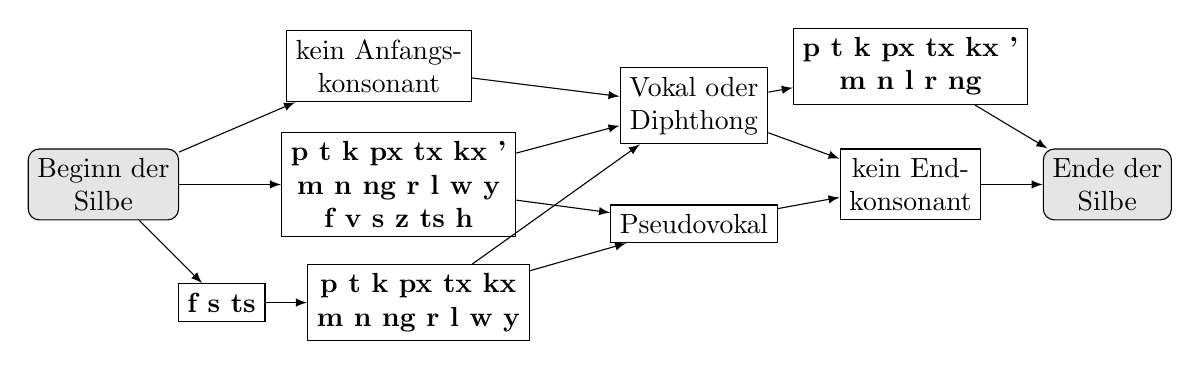
\begin{tikzpicture}[every path/.style={>=latex},every node/.style={draw,rectangle}]
		\node[rounded corners,fill=gray!20,align=center] (sos) at (-4,1) {Beginn der\\Silbe};
		\node[align=center] (zero-onset) at (-0.5,2.5) {kein Anfangs-\\konsonant};
		\node[align=center,font=\bfseries] (onset) at (-0.25,1) {p t k px tx kx '\\ m n ng r l w y\\f v s z ts h};
		\node[font=\bfseries] (clust-c1) at (-2.5,-0.5) {f s ts};
		\node[align=center,font=\bfseries] (clust-c2) at (0,-0.5) {p t k px tx kx\\m n ng r l w y};
		\node[align=center] (vowel) at (3.5,2) {Vokal oder\\Diphthong};
		\node (pseudovowel) at (3.5,0.5) {Pseudovokal};
		\node[align=center,font=\bfseries] (final) at (6.25,2.5) {p t k px tx kx ’\\m n l r ng};
		\node[align=center] (zero-coda) at (6.25,1) {kein End-\\konsonant};
		\node[rounded corners,fill=gray!20,align=center] (eos) at (8.75,1) {Ende der\\Silbe};
		
		\draw[->] (sos) edge (clust-c1);
		\draw[->] (sos) edge (onset);
		\draw[->] (sos) edge (zero-onset);
		\draw[->] (clust-c1) edge (clust-c2);
		\draw[->] (zero-onset) edge (vowel);
		\draw[->] (clust-c2) edge (vowel);
		\draw[->] (clust-c2) edge (pseudovowel);
		\draw[->] (onset) edge (vowel);
		\draw[->] (onset) edge (pseudovowel);
		\draw[->] (vowel) edge (final);
		\draw[->] (final) edge (eos);
		\draw[->] (vowel) edge (zero-coda);
		\draw[->] (pseudovowel) edge (zero-coda);
		\draw[->] (zero-coda) edge (eos);
	\end{tikzpicture}
\end{center}

\subsubsection{} Da eine Silbe nicht unbedingt einen Anfangs- oder Endkonsonanten haben muss, ist es durchaus möglich, dass mehrere Vokale in einem Wort nebeneinander stehen. In diesem Fall ist jeder Vokal eine Silbe für sich, \N{muiä} [mu.i.æ], \N{ioang} [i.o.aŋ].

\subsubsection{} In Allgemeinen wird die Sequenz VKV als V.KV anstelle von VK.V getrennt; so wird \N{tsenge} als [tsɛ.ŋɛ] und nicht als *[tsɛŋ.ɛ] getrennt. Onomatopoie (Lautmalerei) kann dies aufheben, wenn ein Echoeffekt gewünscht ist, wie in \N{kxangangang} [k'aŋ.aŋ.aŋ].

\subsubsection{} Es gibt keine Langvokale im Wald-Na'vi, d. h. identische Vokale kommen nicht nebeneinander vor (siehe aber \horenref{lands:contract}). Das Riff-Na'vi kann aufgrund der Elision des glottalen Plosivs (\horenref{rn:stop-elision}) in verschiedenen Umgebungen lange Vokale haben, auch durch Weglassen der Kontraktion (\horenref{rn:no-contract}).

\subsubsection{} In Grundwörtern treten keine doppelten Konsonanten auf, aber sie können an Morphemgrenzen auftreten, wie z. B. in Ableitungen, \N{tsukkäteng} $<$ \N{tsuk-} $+$ \N{käteng}, oder mit Enklitika \N{Mo'atta} $<$ \N{Mo'at} $+$ \N{ta} (\horenref{lands:stress:enclisis}).
% https://naviteri.org/2011/03/“receptive-ability”-and-hesitation/comment-page-1/#comment-604

\subsubsection{} Wie in vielen menschlichen Sprachen brechen manche Interjektionen diese Regeln, wie etwa \N{oìsss}, ein Laut des Zorns bzw. Ärgers, oder \N{saa}, ein Drohruf.

\subsection{Betonung}
Jedes Na'vi-Wort hat mindestens eine betonte Silbe, die nicht vorhersagbar ist. In sehr wenigen Fällen unterscheiden sich ansonsten identische Wörter nur durch ihre Betonung, beispielsweise \N{\ACC{tu}te} \E{Person} vs. \N{tu\ACC{te}} \E{Frau}.

\subsubsection{} Nur für dieses Wort, \E{Frau}, darf in normalem Na'vi ein Akzent geschrieben werden, um die Betonung anzuzeigen, \N{tuté}.
\index{tuté@\textbf{tuté}}

\subsubsection{} Manche Wortbildungsprozesse können Verschiebungen in der Betonung verursachen (\horenref{lingop:prefix:ke}, \horenref{lingop:suffix:gender}).

\subsubsection{} Alle Adpositionen sowie wenige Konjunktionen und Partikel können en­kli­tisch sein. Sie verlieren dadurch ihre eigene Betonung, werden effektiv Teil des Wortes, an das sie angehängt sind, und daher zusammen geschrieben, \N{\ACC{tsa}ne} ($<$ \N{tsaw} $+$ \N{ne}), \N{ho\ACC{ren}tisì} ($<$ \N{ho\ACC{ren}ti} $+$ \N{sì}).
\label{lands:stress:enclisis}\index{enclitics}

\subsubsection{} Obwohl zusammengesetzte Substantive als ein einziges Wort geschrieben werden, können die einzelnen Bestandteile ihre ursprüngliche Betonung beibehalten, wie in \N{ti\ACC{re}a\ACC{fya}'o} \E{Geistespfad}.\index{compound word!accent}
%\subsubsection{} Word stress is a property of stem words.  No matter
%how many affixes a root word takes, no secondary accents develop.
\subsection{Riff-Na'vi} Der Riff-Na'vi-Dialekt unterscheidet sich sowohl im Konsonantismus als auch im Vokalismus vom Wald-Na'vi. \index{Riff-Na'vi}
\NTeri{8/1/2022}{http://naviteri.org/2023/01/reef-navi-part-1-phonetics-and-phonology/}

\subsubsection{} Ein Ejektiv-Konsonant am Anfang einer Silbe -- und damit am Anfang eines Wortes -- wird im Riff-Na'vi stattdessen als stimmhafter Plosiv ausgesprochen; d. h. \N{px tx kx} → [b d g].

\begin{center}
	\begin{tabular}{lll}
		\N{txon}    & [don] & \E{Nacht} \\
		\N{hol\ACC{pxay}} & [hol.ˈbaj] & \E{Zahl, Nummer} \\
		\N{kxitx}   & [git'] & \E{Tod} \\
		\N{skxawng} & [sk'awŋ] (wie Wald-Na'vi) & \E{Idiot, Trottel}
	\end{tabular}
\end{center}

\noindent Im Allgemeinen wird diese Änderung nicht ausgeschrieben. Das heißt, Riff-Dialekt-Texte schrei-ben \E{Nacht} als \N{txon}, erwarten aber vom Leser das Wissen, dass es \N{don} ausgesprochen wird. Wenn jedoch die Verwendung des Riff-Dialekts betont werden soll, kann es als \N{don} geschrieben werden.

Bei einem Wort wie \N{tìkankxan} führt die Ausschreibung des Riff-Dialekts zur mehrdeutigen Schreibweise \N{*tìkangan}. Um zu vermeiden, dass \N{...ng...} als [ŋ] statt als [ŋg] interpretiert wird, kann ein Interpunkt (bevorzugt) oder ein Bindestrich verwendet werden: \N{tìkan·gan} oder \N{tìkangan}.
\Omaticon{} \NTeri{15/1/2023}{http://naviteri.org/2023/01/2653/\#comment-45092}

\paragraph{} Wenn ein Wort, das mit einem Ejektiv endet, ein Suffix erhält, das mit einem Vokal beginnt, wird die Aussprache des Ejektivs an die neue Silbenstruktur angepasst. Z. B. ist \N{'awkx} mit dem Ejektiv [ʔawk'], aber \N{'awkxit} ist [ʔaw.git], mit der stimmhaften Aussprache.
\NTeri{13/1/2023}{http://naviteri.org/2023/01/2653/}



\subsubsection{} In einem Cluster mit \N{y} palatalisieren \N{s} und \N{ts}.\footnote{\href{https://de.wikipedia.org/wiki/Palatalisierung}{Vgl. Wikipedia: Palatalisierung}} Das bedeutet, \N{sy} wird als [ʃ] und \N{tsy} als [tʃ] ausgesprochen. Aufgrund der Silbenstruktur des Na'vi kann dies nur am Anfang einer Silbe geschehen.

\begin{center}
	\begin{tabular}{lll}
		\N{syaw} & [ʃaw] & \E{rufen} \\
		\N{tsìsyì} & [ˈtsɪ.ʃi] & \E{flüstern} (vin.) \\
	\end{tabular}
\end{center}

\noindent Diese Lautveränderung des Riff-Na'vi wird in der Schreibung nie angegeben.

\subsubsection{} \index{Reef Na'vi!glottal stop elision}\label{rn:stop-elision}
Zwischen zwei Vokalen entfällt der glottale Plosiv im Riff-Na'vi normalerweise. Beide Vokale werden dennoch deutlich ausgesprochen, auch wenn sie identisch sind, wie in \N{rä'ä} unten,

\begin{center}
	\begin{tabular}{lll}
		\N{fra'u} & \N{frau} & \E{alles} \\
		\N{Lo'ak} & \N{Loak} & \E{Lo'ak} (Name einer Person) \\
		\N{rä'ä}  & \N{rää} & \E{tu nicht, mach nicht}
	\end{tabular}
\end{center}

\noindent Diese Veränderung ist bis zu einem gewissen Grad auch im Wald-Na'vi zu beobachten, wie etwa beim Namen \N{Lo'ak} (\horenref{names-with-oa}).

Während der glottale Plosiv am Anfang und am Ende von Wörtern beibehalten wird, kann er bei der Hinzufügung von Affixen, durch die der Plosiv dann intervokalisch steht, entfallen. Z. B. lautet der Ausdruck für \E{humorvolle Person} im Wald-Na'vi \N{tute a'ipu}, aber im Riff-Na'vi \N{tute aipu}; oder das Adverb \E{nur} \N{nìaw} statt, wie im Wald-Na'vi, \N{nì'aw}.
\NTeri{14/1/2023}{http://naviteri.org/2023/01/2653/\#comment-45068}

\subsubsection{}
In unbetonten Silben kann im Riff-Na'vi \N{ä} zu \N{e} werden.

\begin{center}
	\begin{tabular}{lll}
		\N{\ACC{nge}yä} & \N{ngeye} & \E{dein} \\
		\N{tä\ACC{txaw}} & \N{tedaw} & \E{zurückkommen, zurückkehren, wiederkommen} (vin.) \\
		\N{\ACC{kä}}     & \N{kä}  & \E{gehen}
	\end{tabular}
\end{center}

\Omaticon

\subsection{Gesprochenes Alphabet}
Mit Ausnahme von \N{tìftang}, dem glottalen Plosiv, enthalten die Namen der Phoneme Informationen darüber, wie der Laut verwendet wird. Sie werden zudem bei der Ausschreibung ungewöhnlicherweise großgeschrieben: \index{alphabet!spoken}

\begin{center}\small
	\begin{tabular}{lll}
		\N{tìftang} & \N{Ì} & \N{ReR} \\
		\N{A}  & \N{KeK}   & \N{'Rr} \\
		\N{AW} & \N{KxeKx} & \N{Sä} \\
		\N{AY} & \N{LeL}   & \N{TeT} \\
		\N{Ä}  & \N{'Ll}   & \N{TxeTx} \\
		\N{E}  & \N{MeM}   & \N{Tsä} \\
		\N{EW} & \N{NeN}   & \N{U} \\
		\N{EY} & \N{NgeNg} & \N{Vä} \\
		\N{Fä} & \N{O}     & \N{Wä} \\
		\N{Hä} & \N{PeP}   & \N{Yä} \\
		\N{I}  & \N{PxePx} & \N{Zä} \\
	\end{tabular}
\end{center}

\subsubsection{} Vokale und Diphthonge werden einfach als solche ausgesprochen und geschrieben. Die Pseudovokale brauchen einen vorangehenden glottalen Plosiv, da sie einen Anfangskonsonanten benötigen (\horenref{lands:pseudo-no-null}).

\subsubsection{} Die Namen für Konsonanten, die nicht am Silbenende stehen dürfen, werden durch Hinzufügen von \N{ä} gebildet, wie in \N{Tsä}. Diejenigen, die am Silbenende stehen dürfen, verwenden den Vokal \N{e} und wiederholen den Konsonanten am Ende des Namens, \N{PeP}.

\section{Lenition}
\noindent Bestimmte grammatikalische Prozesse führen zu einer Änderung des anlautenden Konsonanten eines Wortes. Diese Veränderung wird als ``Lenition'' (auch ``Lenierung'' oder ``Lenisierung'') bezeichnet\footnote{\href{https://de.wikipedia.org/wiki/Lenisierung}{Vgl. Wikipedia: Lenisierung}}. Nur acht Konsonanten werden leniert.\index{lenition}\label{lands:lenition}
\LanguageLog

\begin{center}
	\begin{tabular}{lll}
		Konsonant & Lenition & Beispiel \\
		\N{px, tx, kx} & \N{p, t, k} & \N{\uwave{tx}ep}, aber \N{mì \uwave{t}ep} \\
		\N{p, t, k} & \N{f, s, h} & \N{\uwave{k}elku}, aber \N{ro \uwave{h}elku} \\
		\N{ts} & \N{s} & \N{\uwave{ts}mukan}, aber \N{ay\uwave{s}mukan} \\
		\N{’} & verschwindet & \N{’eylan}, aber \N{fpi eylan} \\
	\end{tabular}
\end{center}

\noindent In den Zwischenzeilen wird die Lenition bei der morphologischen Aufschlüsselung in der zweiten Zeile entfernt (wie in Beispiel \ref{lenition:ex01} unten).

\subsection{Glottaler Plosiv} Der glottale Plosiv wird nicht leniert, wenn er einem Pseudovokal vor-angestellt ist (\N{mì 'Rrta}, nicht *\N{mì Rrta}).
\index{glottal stop!lenition}\label{lands:lenition:pseudovowel}\NTeri{3/28/2012}{https://naviteri.org/2012/03/spring-vocabulary-part-1/}

\subsection{Adpositionen} Einige wenige Adpositionen verursachen Lenition, wenn sie einem Wort vorausgehen: \N{fpi}, \N{ìlä}, \N{mì}, \N{nuä}, \N{ro}, \N{sko}, \N{sre} (und abgeleitet \N{lisre} und \N{pxisre}), \N{wä}. Als Suffixe bewirken sie weder in dem Wort, an das sie angehängt sind, noch in dem folgenden Wort eine Lenition.
\NTeri{7/7/2010}{https://naviteri.org/2010/07/thoughts-on-ambiguity/}
\index{fpi@\textbf{fpi}!lenition}\index{ilä@\textbf{ìlä}!lenition}
\index{miì@\textbf{mì}!lenition}\index{ro@\textbf{ro}!lenition}
\index{sre@\textbf{sre}!lenition}\index{pxisre@\textbf{pxisre}!lenition}
\index{waä@\textbf{wä}!lenition}\index{nuaä@\textbf{nuä}!lenition}
\index{sko@\textbf{sko}!lenition}
\index{lenition!adpositions}\index{adpositions!lenition}

\subsection{Numeruspräfixe} Präfixe, die Lenition verursachen, werden mit einem Pluszeichen anstelle des üblichen Bindestrichs gekennzeichnet, wie z. B. \N{ay+}, das lenierende Präfix für den Plural.\index{lenition!number prefixes}

\subsection{Fragepronomen} Wenn es als Präfix verwendet wird, verursacht das Fragepronomen \N{pe+} Lenition (\horenref{morph:pre:pe}), wie in \N{pehem} \E{Was? (welche Aktion?)} von \N{kem} \E{Tat, Handlung}.

\subsection{Zahlen}\index{lenition!numbers}
Werden Zahlen als Suffixe verwendet, lenieren abhängige Formen der Zahlen (\horenref{numbers:dependent}), wie in \N{vopey} \E{elf (8 + 3)}, aber \N{pxey} \E{drei}.

\subsection{Eigennamen} Eigennamen werden ebenfalls leniert.

\begin{interlin} \label{lenition:ex01}
	\glll Oe kelku si mì Helutral. \\
	oe kelku si mì Kelutral \\
	\I{1sg} Heim machen in Heimatbaum \\
	\trans{Ich lebe im Heimatbaum}
\end{interlin}

\index{lenition!proper nouns}\NTeri{10/28/2010}{https://naviteri.org/2010/09/getting-to-know-you-part-2/}

\subsection{Riff-Na'vi} \index{Reef Na'vi!lenition}
Obwohl die Ejektive im Riff-Na'vi als stimmhafte Plosive am Anfang eines Wortes auftauchen, gelten die Regeln für die Lenition weiterhin wie im Wald-Na'vi. Das bedeutet, obwohl \N{txon} \E{Nacht} im Riff-Na'vi als \N{don} ausgesprochen wird, ist die lenierte Form immer noch \N{ton}.
\LNWiki{8/1/2023}{http://naviteri.org/2023/01/reef-navi-part-1-phonetics-and-phonology/}

\section{Morphophonologie}

\subsection{Vokalkontraktionen} Da identische Vokale nicht nebeneinander stehen dürfen, gibt es einige grammatikalische Prozesse, bei denen ein doppelter Vokal zu einem einzigen kontrahiert wird.\footnote{\href{https://de.wikipedia.org/wiki/Kontraktion_(Linguistik)}{Vgl. Wikipedia: Kontraktion}}\index{vowel!contraction}\label{lands:contract}

\subsubsection{} Das Adjektivmorphem \N{-a-} verschwindet, sobald es an ein \N{a} am Anfang oder Ende eines Adjektivs angefügt wird, wie in \N{apxa tute}, nicht *\N{apxaa tute}.
\index{-a-@\textbf{-a-}!with \textbf{a} in an adjective}
\index{adjective!contraction}

\subsubsection{} Wenn das Dual- und Trialpräfix zu einer Sequenz mit zwei \N{e} führt wie in \N{me} $+$ \N{'eveng} $>$ *\N{meeveng} (beachte Lenition), dann kontrahieren diese Vokale zu einem einzigen, \N{meveng}.
\label{lands:phonotactics:nsc} \index{dual!contraction}
\index{trial!contraction}\LNWiki{20/1/2010}{https://wiki.learnnavi.org/index.php/Canon\%23Extracts_from_various_emails}

\subsubsection{} Wenn das Präfix auf denselben Vokal endet wie der, mit dem das folgende Wort beginnt, kontrahieren sie zu einem einzigen Vokal, wie in \N{tsatan} $<$ \N{tsa-} $+$ \N{atan}, \N{fìlva} $<$ \N{fì-} $+$ \N{ìlva} (\horenref{morph:prenoun:contraction}).\footnote{Der glottale Plosiv ist ein Konsonant, daher kontrahiert \N{ì} in \N{fì'ìheyu} (von \N{fì-} $+$ \N{'ìheyu}) nicht.}
\label{lands:phonotactics:precontract}\index{prenoun!contraction}\LNWiki{18/5/2011}{https://wiki.learnnavi.org/index.php/Canon/2011/April-December\%23Kawtseng.2C_tsapo_and_prefixes}

\subsubsection{} Kontraktion kommt beim Indefinitsuffix \N{-o} oder enklitischen Adpositionen nicht vor. Wenn zwei identische Vokale nebeneinander stehen, werden sie mit einem Bindestrich dazwi-schen geschrieben: \N{fya'o-o} \E{irgendeine Weise}, \N{zekwä-äo} \E{unter einem Finger}.\footnote{Obwohl das Wald-Na'vi technisch gesehen keine Langvokale hat, tritt der Effekt der Langvokale aus dem Riff-Na'vi (\horenref{rn:stop-elision}) in dieser Situation auf. Man beachte also die Aussprache beider \N{ä} in einem Wort wie \N{zekwä-äo}.}\index{vowel!contraction!inhibited}
% https://wiki.learnnavi.org/index.php/Canon/2010/UltxaAyharyuä#Phonological_Questions

\subsubsection{} Im Riff-Na'vi wird die Vokalkontraktion nicht angewendet. Formen wie \N{meeveng} oder \N{apxaa} bleiben bestehen, während das Wald-Na'vi die doppelten Vokale kontrahieren würde.
\index{Reef Na'vi!vowel contraction inhibited}\label{rn:no-contract}\NTeri{13/1/2023}{http://naviteri.org/2023/01/2653/}

\subsection{Pseudovokalkontraktion} Aufgrund der Form der Aspektinfixe \N{\INF{er}} und \N{\INF{ol}} ist es möglich, dass die Pseudovokale unmittelbar nach ihrem konsonantischen Gegenstück auftreten, wie in \N{*p\INF{ol}ll\ACC{txe}}. Wenn dies in einer unbetonten Silbe geschieht, verschwindet der Pseudovokal, \N{pol\ACC{txe}}. In einer betonten Silbe verschwindet das Infix, \N{*\ACC{f}\INF{er}\ACC{rr}fen} $>$ \N{\ACC{frr}fen}. Pseudovokale in einsilbigen Wörtern verhalten sich wie unbetont, \N{vol} von \N{*v\INF{ol}ll}. \index{pseudovowel!contraction}
\LNWiki{23/3/2010}{https://wiki.learnnavi.org/index.php/Canon/2010/March-June\%23Misc_Answers}
\NTeri{19/6/2012}{https://naviteri.org/2012/06/spring-vocabulary-part-3/}

\subsection{Affektinfix-Epenthese} Wenn auf das positive Affektinfix \N{\INF{ei}} der Vokal \N{i}, \N{ì} oder ein Pseudovokal folgt, wird ein \N{y} eingefügt (Epenthese\footnote{\href{https://de.wikipedia.org/wiki/Epenthese}{Vgl. Wikipedia: Epenthese}}):\\ \N{seiyi} $<$ \N{*s\INF{ei}i}, \N{veykrreiyìn} $<$ \N{*veykrr\INF{ei}ìn}; \N{v\INF{ei}yll} $<$ \N{*veill}.
\label{lands:eiy-epenth}
\NTeri{19/6/2012}{https://naviteri.org/2012/06/spring-vocabulary-part-3/}

\subsubsection{Riff-Na'vi} \index{Reef Na'vi!affect infix epenthesis}
Die Dissimilation von \N{seii} zu \N{seiyi} kommt im Riff-Na'vi nicht vor.
\NTeri{31/1/2023}{http://naviteri.org/2023/01/2653/}


\subsection{Assimilation des stimmhaften Plosivs im Riff-Na'vi} \index{Reef Na'vi!voiced stop assimilation}
Wenn ein Wort im Riff-Na'vi einen Ejektiv-Cluster enthält, wie z. B. in \N{atxkxe} \E{Land}, findet eine regressive stimmhafte Assimilation statt.
Das bedeutet, dass der stimmhafte Plosiv am Silbenanfang (*\N{atxge}) auch die Stimmhaftigkeit des  Ejektivs am Ende der vorhergehenden Silbe verursacht, was zu \N{adge} führt.
In ähnlicher Weise wird \N{ekxtxu} \E{rau, grob} zu \N{egdu} im Riff-Na'vi.
\LNWiki{8/1/2023}{http://naviteri.org/2023/01/reef-navi-part-1-phonetics-and-phonology/}

\subsection{Nasale Assimilation} In vielen Komposita sowie in einigen Idiomen passen sich finale Nasallaute an die Artikulationsposition des Konsonanten im Anlaut des folgenden Wortes an, wie in \N{lumpe} als Variante von \N{pelun}. Eine solche Assimilation wird nicht immer geschrieben, wodurch die Etymologie eines Wortes deutlicher werden kann, wie in \N{zenke} anstelle von \N{*zengke}, von \N{zene ke}; oder in den verschiedenen Idiomen mit dem Verb \N{tìng} \E{geben}, wobei \N{tìng mikyun} als \N{tìm mikyun} ausgesprochen wird. \index{nasal assimilation} \label{lands:nasalassim}

\subsection{Vokalharmonie} In Na'vi gibt es zwei Fälle von optionaler regressiver Vokalharmonie in Verbinfixen.\index{vowel!harmony}

\subsubsection{} Das subjunktivische Futur-Infix, \N{\INF{iyev}}, erscheint am häufigsten als \N{\INF{ìyev}}, mit einer Senkung des ersten Vokals.

\subsubsection{}\label{lands:eng}
Der Vokal des negativen Affektinfixes, \N{\INF{äng}}, kann gehoben werden, wenn es unmittelbar von dem Vokal \N{i} gefolgt wird, wodurch es zu \N{\INF{eng}} wird,

\begin{interlin}
	\glll Tsap'alute sengi oe. \\
	tsap'alute s\INF{äng}i oe \\
	Entschuldigung machen\INF{\I{neg.aff}} \I{1sg} \\
	\trans{Ich entschuldige (mich).}
\end{interlin}

\Ultxa{2/10/2010}{https://wiki.learnnavi.org/index.php/Canon/2010/UltxaAyharyu\%C3\%A4\%23.C3.A4ng.2Feng}

\subsection{Elision} In schneller Rede entfällt finales \N{-e} häufig (Elision\footnote{\href{https://de.wikipedia.org/wiki/Elision}{Vgl. Wikipedia: Elision}}), wenn das darauf folgende Wort mit einem Vokal beginnt, \Npawl{Kìyevam$\not$e ult$\not$e Eywa ngahu}. Dies wird in der Schrift nicht angegeben.\index{elision}
Steht das finale \N{-e} in einem einsilbigen Worte (\N{ke, sre}), oder ist es betont (\N{tuté}), entfällt es nicht.
\LNForum{25/10/2022}{https://forum.learnnavi.org/index.php?msg=679687}

\subsubsection{} Der Vokal \N{ì} in \N{mì}, \N{sì} und dem Adverbpräfix \N{nì-} entfällt vor dem Pluralpräfix \N{ay+}, obwohl sich die Schreibung nicht ändert. So wird \N{nìayfo} \E{wie sie} als \N{nayfo} ausgesprochen.\label{lands:elision-i}\index{miì@\textbf{mì}!elision with plural}\index{siì@\textbf{sì}!elision with plural}\index{niì-@\textbf{nì-}!elision with plural}
\NTeri{1/7/2010}{https://naviteri.org/2010/07/thoughts-on-ambiguity/}

\subsubsection{} Der Vokal in \N{nì-} entfällt normalerweise vor einem betonten \N{e}, wie in \N{nì-} $+$ \N{etrìp} $>$ \N{netrìp}. Wenn das \N{e} unbetont ist, entfällt es normalerweise, wenn auch nicht immer, ebenfalls, \N{nì-} $+$ \N{eyawr} $>$ \N{nìyawr}. Eine Ausnahme: \N{nìean} statt des erwarteten \N{*nìan}.
\index{niì-@\textbf{nì-}!elision before e}
\LNForum{9/8/2017}{https://forum.learnnavi.org/index.php?msg=595528}

\subsection{Andere phonetische Prozesse}

\subsubsection{Namen mit -o'a-} \label{names-with-oa}
In der Umgangssprache kann bei Namen, die die Sequenz \N{o'a} enthalten, der glottale Plosiv entfallen, wie z. B. \N{Mo'at} \textasciitilde{} \N{Moat} und \N{Lo'ak} \textasciitilde{} \N{Loak}.
\NTeri{1/3/2017}{https://naviteri.org/2017/02/ayioang-amip-si-ayu-alahe-new-animals-and-other-things/\#comment-26401}

\section{Orthographische Konventionen}
\noindent Na'vi folgt im Allgemeinen in Bezug auf Schreibung, Interpunktion und Kapitalisierung den orthographischen Gewohnheiten des Englischen, aber es gibt einige Unterschiede.

\subsection{Eigennamen} Wenn sie mit lexikalischen Präfixen (\horenref{lingop:affixes}) versehen werden, behalten Eigennamen ihre ursprüngliche Großschreibung bei, wie in \N{lì'fya le\uwave{Na'vi}}.

\subsection{Zitation} Direkte Rede wird im Na'vi nicht mit Anführungszeichen gekennzeichnet. Stattdessen wird auf die Zitationspartikel \N{san\dots sìk} (siehe \horenref{syn:direct-quote}) zurückgegriffen.
\index{quotation!punctuation}

\subsection{Etymologische Schreibweise} Neben der gelegentlichen Schreibweise von Nasalen, wel-che die Etymologie widerspiegelt (\horenref{lands:nasalassim}), gibt es einige grammatikalische Prozesse, die zu einer Schreibweise führen, die eher die Grammatik als die Aussprache hervorheben.

\subsubsection{} Das Grundwort des Pronomens der ersten Person \N{oe} wird zwar als \N{we} ausgesprochen, wenn es ein Suffix erhält, behält aber die ursprüngliche Schreibweise bei
(\horenref{morph:pron:oe-we}).

\subsubsection{} Vor Wörtern, die mit \N{y} beginnen, bleibt das Pluralpräfix \N{ay+} unverändert, wie beispielsweise bei \N{ayyerik}.
\LNWiki{18/4/2010}{https://wiki.learnnavi.org/index.php/Canon/2010/March-June\%23ay.2Byerik}

\subsection{Attributivphrasen mit Bindestrich} Bestimmte kurze Attributivphrasen werden mit Bindestrichen geschrieben, welche die Elemente verbinden.

\subsubsection{} Attributivphrasen mit Farbadjektiven, die \N{na} \E{wie} verwenden, werden mit Bindestrichen geschrieben, \N{fìsyulang aean-na-ta'leng} \E{diese hautblaue Blume} (\horenref{syn:attr:na}).

\subsubsection{} Partizipien von \N{si}-Verben werden ebenfalls mit Bindestrich geschrieben, \N{srung-susia tute} \E{eine helfende Person}
(\horenref{syn:participle:si-const}).